\section{Classic Cracking}
\label{sec:classic-cracking}
\emph{Database Cracking} is a pleasantly simple approach to adaptive
indexing.  However, it is not trivial to implement efficiently. In this
section, we recapitulate the original \emph{Cracking} algorithm and we
examine the problems with the current implementation regarding CPU
efficiency.

\subsection*{The Algorithm}
\label{sec:algorithm}

\begin{figure}[!t]
\begin{center}
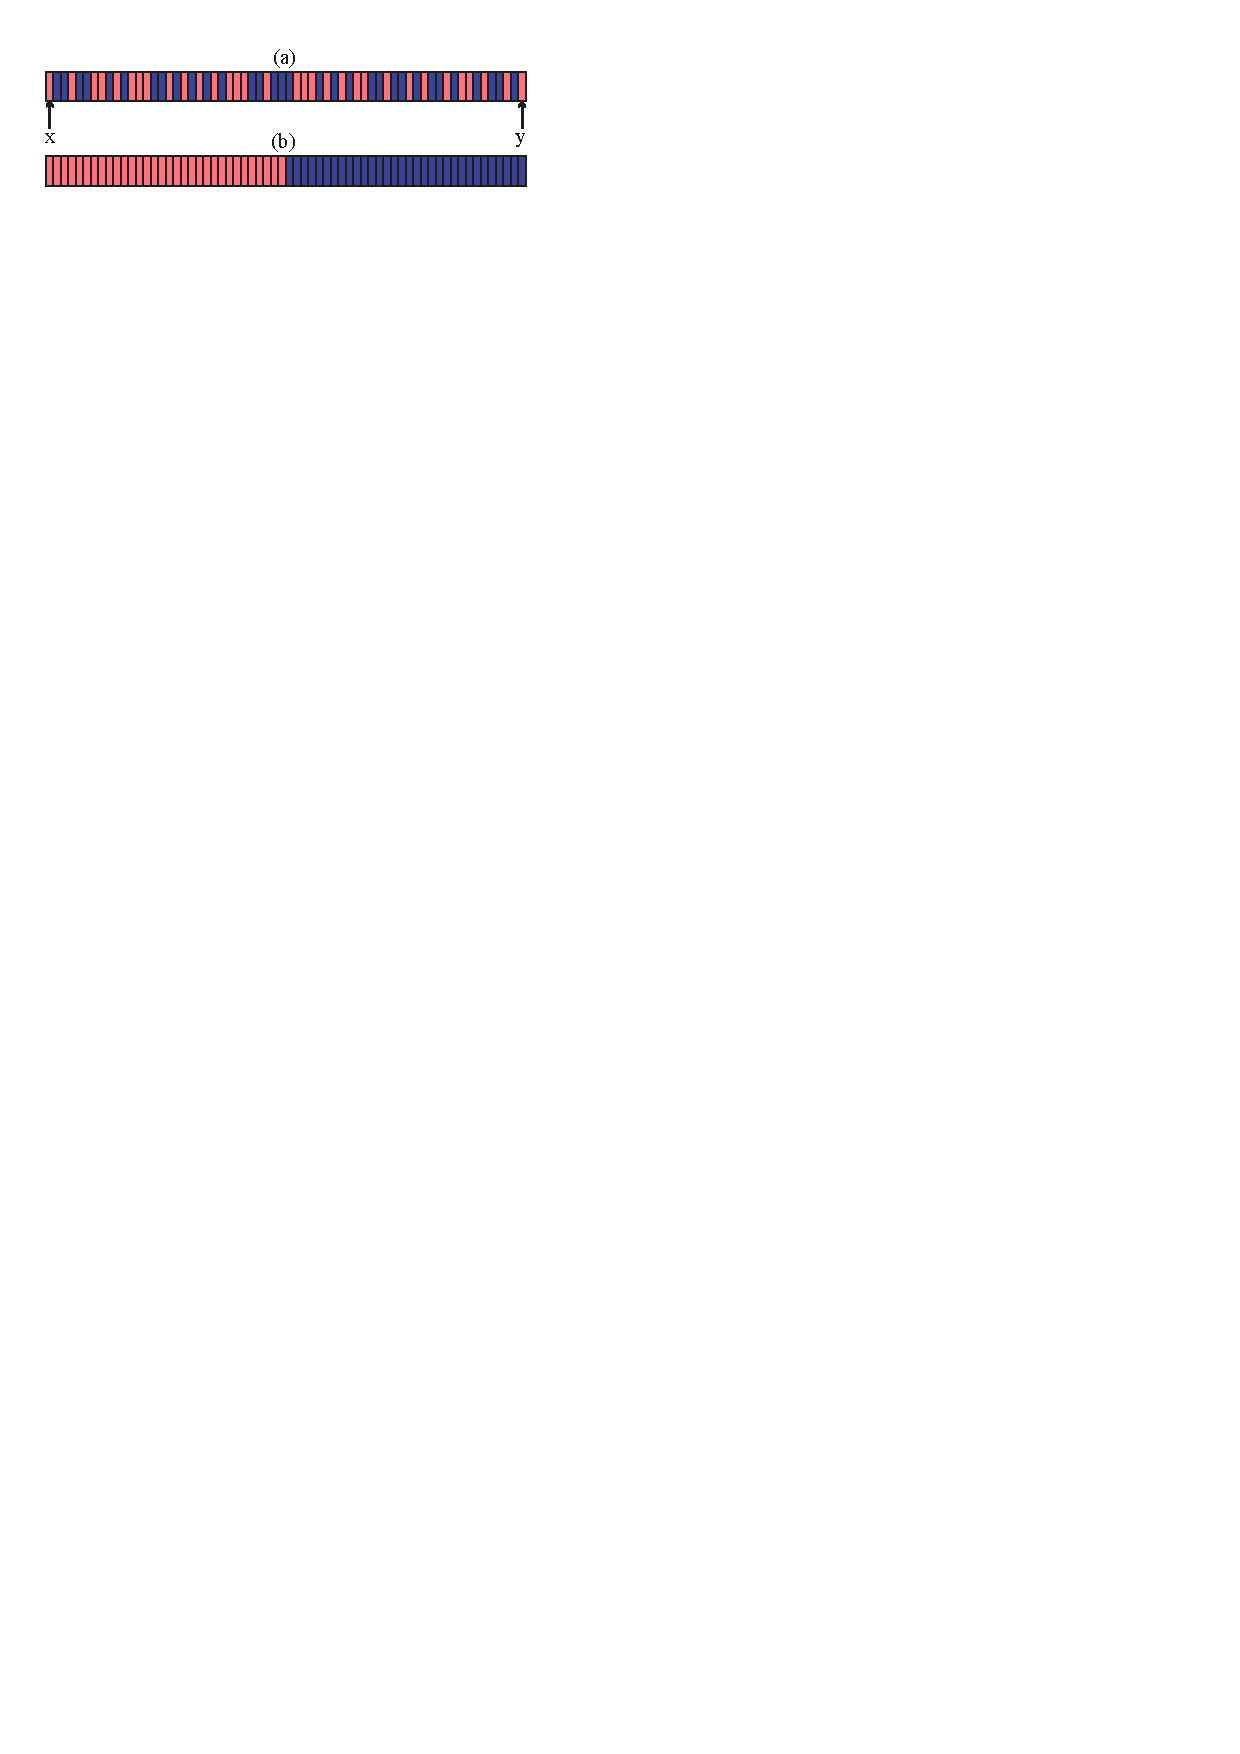
\includegraphics[trim=0.6cm 26.7cm 0cm 1cm]{Figures/damon/naive}
\vspace{-0.2 in}
\caption{Original Cracking (single-threaded)}
\vspace{-0.37 in}
\label{fig:naive}
\end{center}
\end{figure}

\begin{figure*}[t]
    \centering
  \subfloat[Cache Misses]{
    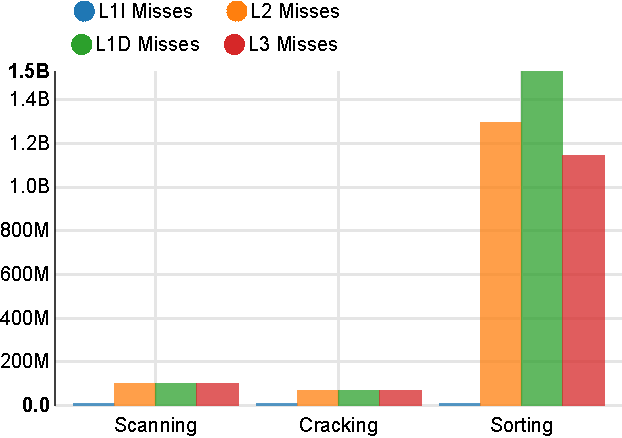
\includegraphics[width=.85\columnwidth]{Figures/damon/AnalysisCacheMisses}
\hspace{.05\columnwidth}
    \label{fig:cracking-cache-misses}
  }
  \subfloat[Costs breakdown by CPU component]{
\hspace{.05\columnwidth}
    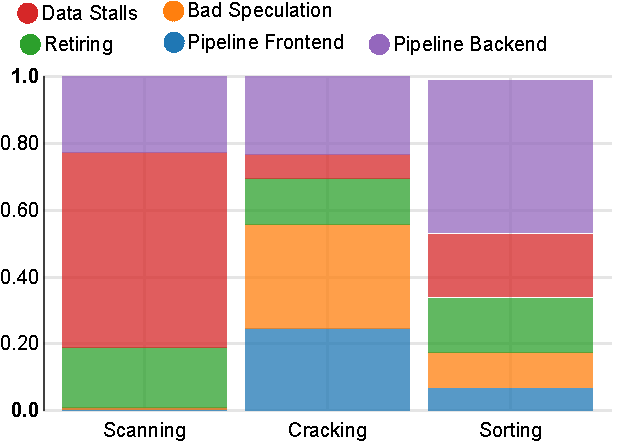
\includegraphics[width=.85\columnwidth]{Figures/damon/CostBreakdown}
    \label{fig:cracking-non-load-stalling}
  }
  \label{fig:cracking-cost-breakdown}
  \caption{Cost Breakdown of Database Operations}
\vspace{-0.2 in}
  \centering
\end{figure*}


The original, single-threaded \emph{Cracking} algorithm is illustrated
in Figure~\ref{fig:naive}.
%that is formally described in Algorithm~\ref{alg:st_cracking}.  
Figure~\ref{fig:naive}(a) depicts an uncracked piece.  Red indicates
values that are lower than the pivot, while blue indicates values that
are greater than the pivot.  Two cursors, $x$ and $y$, point at the
first and at the last position of the piece respectively.  The cursors
move towards each other, scanning the column, skipping values that are
in the correct position while swapping wrongly located values.  The
result of this process is the cracked piece shown in
Figure~\ref{fig:naive}(b).  Values that are less/greater than the
pivot finally lie in a contiguous space.  To crack a piece that
consists of $n$ values, % and a pivot in the middle.
the two cursors read all $n$ values while moving towards each other
resulting in $O(n)$ complexity in terms of computation as well as
memory access.  Thus, \emph{Cracking} and \emph{Scanning} are in the
same complexity class but have significantly different costs (recall
Figure~\ref{fig:motivation}).


\subsection*{Analysis}
\label{sec:analysis}
The classic way of analyzing in-memory data management system
performance is to count the number of cache misses at different
levels. This stems from the assumption that data management
performance is dominated by data access costs. However, as displayed
in Figure~\ref{fig:cracking-cache-misses}, the number of cache misses
do not provide an explanation for the performance difference of
\emph{Cracking} and scanning. In fact, scanning induces more cache
misses because it produces the result set out of place. This indicates
that merely looking at the number of cache misses is not sufficient -
we have to determine the costs induced in other components of the CPU.

To do so, we conducted a systematic analysis of the costs component
according to the Intel optimization manual for our (Ivy Bridge)
CPU~\cite{intelOptimizationManual}. The breakdown in Figure~\ref{fig:cracking-non-load-stalling} shows that
\emph{Cracking} merely spends 7\% of the cycles stalling because of
data access latencies. This explains why the number of cache misses
alone is a poor predictor for the overall performance. The other cost
factors, however give a much better explanation of the performance
difference between \emph{Cracking} and scanning~\footnote{In this
  normalized plot, equal height bars indicate an absolute difference of
  almost factor 10, Figure~\ref{fig:motivation} providing the scale}:
The breakdown shows that 14\% of the cycles~\footnote{or, more
  accurately microop execution slots} are spent retiring (useful)
instructions at the end of the execution pipeline. Assuming that all
instructions are necessary, this indicates that \emph{Cracking} spends
almost 10 times as much CPU cycles as scanning doing actual work. It
also gives us an upper bound on the performance that can be achieved
using a single CPU core: 14\% of the current runtime, i.e., a speedup
factor of about 7. Most importantly, however, this breakdown indicates
where there is most potential for performance improvement: in
eliminating branch mispredictions which
\begin{inparaenum}
\item cause a significant amount of wasted cycles due to \emph{bad speculation} and
\item prevent instructions from entering the \emph{pipeline} at the
  \emph{frontend}.
\end{inparaenum}


